\documentclass[conference]{IEEEtran}
\IEEEoverridecommandlockouts
% The preceding line is only needed to identify funding in the first footnote. If that is unneeded, please comment it out.
\usepackage{cite}
\usepackage{amsmath,amssymb,amsfonts}
\usepackage{algorithmic}
\usepackage{graphicx}
\usepackage{textcomp}
\usepackage{xcolor}
\usepackage{array}
\def\BibTeX{{\rm B\kern-.05em{\sc i\kern-.025em b}\kern-.08em
    T\kern-.1667em\lower.7ex\hbox{E}\kern-.125emX}}
\begin{document}

\title{Explainable Artificial Intelligence \\ {Methodology for Handwritten Applications}}

\author{\IEEEauthorblockN{Paul Whitten, Francis Wolff, Chris Papachristou}
\IEEEauthorblockA{\textit{Electrical, Computer, and Systems Engineering} \\
\textit{Case School of Engineering} \\
\textit{Case Western Reserve University} \\
Cleveland, OH, USA \\
pcw@case.edu, fxw12@case.edu, cap2@case.edu}

}

\maketitle

\begin{abstract}
There has been explosive growth of practical AI in recent years.
%However, inferential results of AI systems are not readily explainable to humans.
A major concern of current AI systems is an inability to explain inferential decisions.
%Explainable artificial intelligence has been posed to mitigate these concerns.
This work explores an Explainable Artificial Intelligence (XAI) methodology that provides explanations
for classification decisions.  Experimental results using the MNIST handwritten digit database are provided with explainable conclusions.
\end{abstract}

\begin{IEEEkeywords}
explainable, artificial intelligence, machine learning
\end{IEEEkeywords}

\section{Introduction}

Recent advances in Machine Learning (ML) have brought about wide adoption of ML algorithms for many applications.  Despite various successes, there is a reluctance to adopt ML in some applications because ML behaves like a black box, decision making by the black box is often not explainable to humans.  

This work approaches the widely studied problem of classifying images of handwritten digits into the ten decimal digit classes, zero through nine, from an Explainable Artificial Intelligence (XAI) perspective.  Our goal is to provide explainable ML classification, in the form of rationale, for classification decisions.  This is achieved using an architecture, with fine-grained classification decisions based on properties, and methodology for constructing an explainable architecture.  Explainability is designed into and is an active component of our proposed architecture\cite{Arrieta2020ExplainableAI}.  While we approach XAI for a specific classification problem, in the MNIST handwritten digit database, the methodology translates to other challenges requiring explainable classification among a finite set of classes.

This work aims to pose a means of explaining classification to a human.  We do not wish to compete with established algorithms that perform exceptionally well in classification of input \cite{keysers07} \cite{lecun98} \cite{schm2012}.  The effort required in applying the methodology in this work is significant compared to training a classifier that will act as a black box, and therefore not be explainable.

\section{Related work}

The ability to map the learning classifier or recognizer to human-based explainability is a challenging task for human understandability.  Currently, there are at least seventeen explainable techniques such as
decision tree-based, rule-based (i.e. knowledgebase), salience mapping,
sensitivity-based analysis, feature importance, fuzzy-based, neural-network, and generic-programming based.  These techniques use one of three basic evaluation approaches: application-grounded, human-grounded and functionally grounded. \cite{BlackBox18} \cite{Arrieta2020ExplainableAI} \cite{Survey18} \cite{Fuzzy19} \cite{Hagras18}  \cite{GP18}

Distributed and fault tolerant systems research has provided several examples of voting \cite{avizienis} and probabilistic models for the voting problem \cite{blough}.

\section{Overview}

 \begin{figure}[htbp]
\centerline{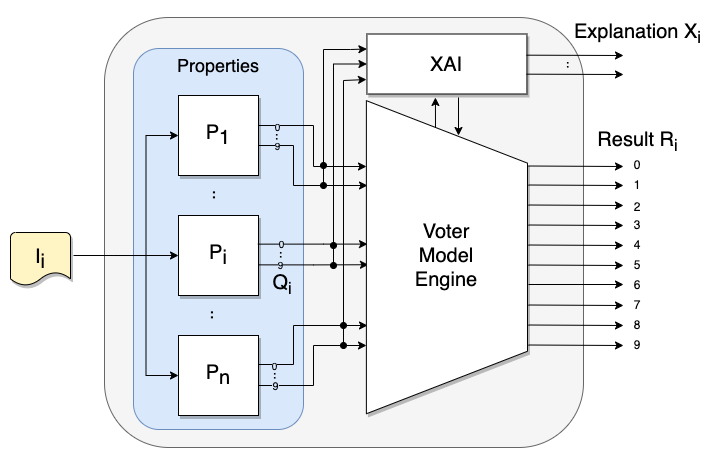
\includegraphics[width=95mm]{./images/voting_prop_nn_2.png}}
\caption{XAI Architecture Summary}
\label{voting}
\end{figure}

The methodology for explainability is based upon the use of explainable properties and related transformations of the input to make distinct classification decisions for each property.  Those distinct classifications are input to a voter to provide a classification decision.  Rationale for the decision is composed from explainable property classifications and combined with the voter result to provide an explanation. 

The explainable architecture used in this work is depicted in Fig.~\ref{voting}.  $I_i$ represents the $i$th input to the architecture.  The architecture consists of Properties, a Voter Model Engine, and an Explainable Artificial Intelligence block.   Explainable properties are defined as descriptive qualities of a sample input that mean something to a user in the problem domain, especially to justify a classification decision.   Explainable properties $P_1$ through $P_n$ are outlined in the blue Property rectangle.  Each property represents logic for a classification based solely on the property.   $Q_i$ represents the $i$th property's classification output.

The Voter Model Engine relies on classifications from the explainable properties, $Q_i$, and feedback from the XAI block to make a final classification decision.   We explore two voting model schemes detailed in \ref{subsection:Voting}.

The XAI block consists of a knowledgebase and logic to generate an explanation for the user.  Inputs to the XAI block are explainable property classifications, $Q_i$, and the Voter Model Engine decision.  The XAI knowledgebase contains information on explainable properties,  a store of training results, and metrics related to the effectiveness of properties.  The explanation provided by the XAI block consists of rationale that relate to the explainable properties contributing to the classification decision.

 \begin{figure}[htbp]
\centerline{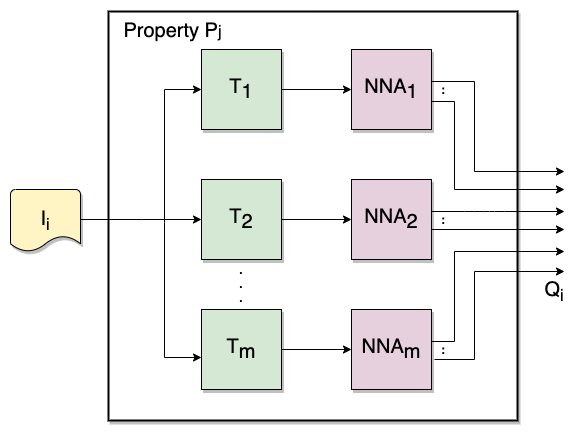
\includegraphics[width=90mm]{./images/property_transforms.png}}
\caption{Architecture of a single property for multiple transformations.}
\label{proptrans}
\end{figure} 

A property transformation is a modifying function applied to the input.  Transformations are used to highlight the explainable property.  Each property may have one or more transformations.   This is represented in Fig.~\ref{proptrans} where the outer square represents the $i$th property square from Fig.~\ref{voting}.  The boxes labeled $T_x$ indicate the $x$th transformation of the input.  Transformed input is fed to a trained Neural Network Architecture (NNA) to make classification decisions.  Classification output then flows to the voter model engine as shown in Fig.~\ref{voting}.

\section{Methodology}
 
Our methodology for achieving explainable ML classification involves the following steps:
%\begin{itemize}
%\item Discover explainable properties.
%\item Define transformations for explainable properties.
%\item Transform training data.
%\item Produce trained explainable property-specific NNAs.
%\item Build a Knowledgebase across the explainable properties.
%\item Devise a voting scheme.
%\item Use a test dataset to provide feedback.
%\end{itemize}

\subsubsection{Discover Explainable Properties}
An explainable property is an attribute of a sample in the problem domain that may differentiate classes and provide a rationale for classification.  This step may require manual analysis of sample inputs to identify properties.

\subsubsection{Define and Implement Transformations}
Data transformations are next defined and implemented to highlight explainable properties in the input.  Transforms may be known algorithms of feature detection and extraction that relate to explainable properties.  In the MNIST example, we used digital image processing techniques such as the morphological skeleton, Hough Circle \& Line Transforms, and flood fill.

\subsubsection{Transform Training Data} 
We next generate a transformed training dataset by submitting all elements from the original training set to the property transformations.  The output from each property transformation is stored for training each property transform specific NNA. 

\subsubsection{Produce Trained Property NNAs}
The next step involves initializing unique NNAs representing each property transformation and then using supervised ML techniques to train the NNAs using only the output of that particular property transform and the original labels.  This results in trained NNAs for each explainable property transform.

\subsubsection{Build an XAI Knowledgebase}
After training, we again process the training set and populate the XAI knowledgebase with the property classification results.  The knowledgebase stores information on properties, the original training label, and each property's classification result.  Metrics on the effectiveness of each explainable property for classes are also calculated and stored in the knowledgebase.  The knowledgebase is used in providing feedback to the voter as well as for composing the classification rationale.

\subsubsection{Devise a Voting Scheme}
We next devise a voting strategy in the Voter Model Engine.  Voting is based on information from the knowledgebase.  The purpose for the voting scheme is to select among the potentially conflicting votes from the explainable property transformation classifications.

\subsubsection{Provide User Feedback}
Finally, when test data is presented to the architecture, we evaluate the results and determine if they are sufficient or if more explainable properties or transforms are needed.

\section{Approach}

This section presents the approach of applying the methodology to the MNIST handwritten digit database. 

\subsection{1 and 2 Properties and Transformations}

We identified explainable properties related to shapes and characteristics of the digits in MNIST.  Fig.~\ref{transsample} depicts the explainable properties and corresponding transformations to identify those properties.  The figure also shows example MNIST digits, $I_i$, and their resulting transforms, $T_i$.

\bgroup
\renewcommand{\arraystretch}{1.8}
%\setlength\tabcolsep{2mm}
\begin{figure}
\centering
\begin{tabular}{ c | p{0.23\linewidth} | p{0.23\linewidth} | ccc | }
\cline{2-6}
& Property & Transform & $I_i$ &  &  $T_i$ \\
\hline \hline
$P_1$ & Stroke & Skeleton & \raisebox{-.5\height}{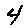
\includegraphics[width=8mm]{./digit-images/4-11.png}} & $\rightarrow$ & \raisebox{-.5\height}{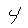
\includegraphics[width=8mm]{./digit-images/4-11-skel.png}} \\
\hline
$P_2$ & Circle & Hough Circle & \raisebox{-.5\height}{
\includegraphics[width=8mm]{./digit-images/6-17.png}} & $\rightarrow$ & \raisebox{-.5\height}{
\includegraphics[width=8mm]{./digit-images/6-17-circle.png}} \\
\hline
$P_3$ & Crossings & Crossings & \raisebox{-.5\height}{
\includegraphics[width=8mm]{./digit-images/4-2.png}} & $\rightarrow$ & \raisebox{-.5\height}{
\includegraphics[width=8mm]{./digit-images/4-2-crossing.png}} \\
\hline
$P_4$ & Circle & Hough Ellipse & \raisebox{-.5\height}{
\includegraphics[width=8mm]{./digit-images/0-3.png}} & $\rightarrow$ & \raisebox{-.5\height}{
\includegraphics[width=8mm]{./digit-images/0-3-ellipse.png}} \\
\hline
$P_5$ & Circle & Multiple Ellipse Circle & \raisebox{-.5\height}{
\includegraphics[width=8mm]{./digit-images/8-4.png}} & $\rightarrow$ & \raisebox{-.5\height}{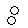
\includegraphics[width=8mm]{./digit-images/8-4-ellipse-circle.png}} \\
\hline
$P_6$ & Endpoints & Endpoints & \raisebox{-.5\height}{
\includegraphics[width=8mm]{./digit-images/2-2.png}} & $\rightarrow$ & \raisebox{-.5\height}{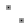
\includegraphics[width=8mm]{./digit-images/2-2-endpoint.png}} \\
\hline
$P_7$ & Enclosed Region & Flood Fill & \raisebox{-.5\height}{
\includegraphics[width=8mm]{./digit-images/0-2.png}} & $\rightarrow$ & \raisebox{-.5\height}{
\includegraphics[width=8mm]{./digit-images/0-2-fill.png}} \\
\hline
$P_8$ & Line & Hough Line & \raisebox{-.5\height}{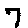
\includegraphics[width=8mm]{./digit-images/7-20.png}} & $\rightarrow$ & \raisebox{-.5\height}{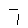
\includegraphics[width=8mm]{./digit-images/7-20-line.png}} \\
\hline
$P_9$ & Enclosed Region & Skeleton Flood Fill & \raisebox{-.5\height}{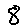
\includegraphics[width=8mm]{./digit-images/8-3.png}} & $\rightarrow$ & \raisebox{-.5\height}{
\includegraphics[width=8mm]{./digit-images/8-3-skel-fill.png}} \\
\hline
\end{tabular}
\centering
\caption{Properties and transforms for the MNIST example}
\label{transsample}
\end{figure}
\egroup

The Stroke property is meant to represent the minimal path of the writing implement to trace the digit.  The morphological skeleton transformation is a one pixel connected representation of the digit, providing a representation of the stroke.  We utilized the Lee\cite{Lee1994} algorithm for obtaining the skeleton.
$P_2$, $P_4$, and $P_5$ are the circle property with corresponding transforms $T_2$, $T_4$, and $T_5$ representing the Hough Circle, the Hough Ellipse, and multiple non-overlapping circles and ellipse transforms respectively.
$P_3$ and $T_3$ are the crossings property and transform representing the intersection of line segments in a digit.  $T_3$ involves taking the skeleton and then finding activated pixels with more than two neighbors.   The endpoints property and transform, $P_6$ and $T_6$, involved taking activated pixels in the skeleton with only one neighbor.
Property $P_7$ and $P_9$ for enclosed regions used transform $T_7$ which involved a flood fill and $T_9$ the flood fill of the skeleton.  The line property and transform, $P_8$ and $T_8$, uses an algorithm to find the non-overlapping Hough Lines of a digit.

\subsection{3, 4, and 5 Transforming, Training, and Knowledgebase}

The various transforms were applied to the MNIST data using implementations in the Python scikit-image library.  The trained NNAs were implemented using scikit-learn Multi-Layer Perceptrons.  The knowledgebase was represented as JSON loaded to in-memory maps for efficient runtime access.

\subsection{6 Voting Schemes}
\label{subsection:Voting}

The first voting scheme we present is probabilistic.  In this scheme, we use a knowledgebase to identify each explainable property transformation's effectiveness to correctly predict a class.   The effectiveness for an explainable property transformation, $i$, to select a particular class, $x$,  is given by:

\begin{equation}\label{effectiveness}
E_{i,x}  = \frac{|A|}{|B|}
\end{equation}

where $A$ is the set of correct classifications of explainable property transformation $i$ of the class $x$ and $B$ is the set of elements of class $x$. 

We take the weight of the effectiveness for each class, $x$, as:
\begin{equation}\label{weight}
W_x=\sum_i E_{i, x}
\end{equation}

The confidence $C_x$ for the class $x$ is given by:

\begin{equation}\label{conf}
C_x=\frac{W_x}{\sum\limits_jW_j}
\end{equation}

The denominator is the sum of all weights for classes that were selected by a property.  If multiple classes are selected by the properties, the class with the highest confidence will be chosen by the voter.

The second voting scheme was NN based.  We utilized explainable property transformation output and labels from MNIST to train a NN in the voter model engine.

\subsection{7 Feedback}

When evaluating early results, there was particular difficulty with the circle transforms for some digits.  The ellipse proved better in generally matching handwritten loop like features.  The single circle transforms worked well for detecting digits zero, six, and nine but performed rather poorly for eight.  Adding a transform that used multiple non-overlapping circles or ellipses was an improvement for eight.  We experimented with the inflection points property and corner detection transforms but the classification results were poor for all digit classes so they were dropped.

\section{Examples}

Detailed examples from MNIST follow in this section by first providing property aggregate classification results for the digits five and six and then explainable results from three different input images will be presented.

Tables ~\ref{table:digit5out} and ~\ref{table:digit6out} show the property transformation NNA output and statistics for properties for digits five and six.  The tables represent the results from processing all of the digits labeled five and six.  The first row of the tables represents effectiveness, $E_{i,x}$.  The second, third and fourth rows represent the standard deviation, kurtosis, and skew of the digit outputs for each property, respectively.  The numbered rows in the tables represent the means of the property outputs for each digit.  The last two rows are the false positive and false negative rates.

We observe that the Stroke property, $P_0$, performed very well in both digits.  The next highest performing property in both tables was the endpoint property, $P_5$, with 85.4\% and 93.3\% accuracy.  The digit six also had good classification results for the enclosed region properties, $P_7$ and $P_9$, due to enclosed regions in the digit six.  The digit six also performed better than the five in the properties related to the circle, $P_2$, $P_4$, and $P_5$.

The digit five had among the poorest performance as observed in the relatively low percent correct and high false negative rates in Table. ~\ref{table:digit5out}.

The mean digit values from the Property NNAs are also represented  in Fig.~\ref{digit5votes} and ~\ref{digit6votes} as three dimensional surface plots for digits five and  and six.

\begin{figure}[htbp]
\centerline{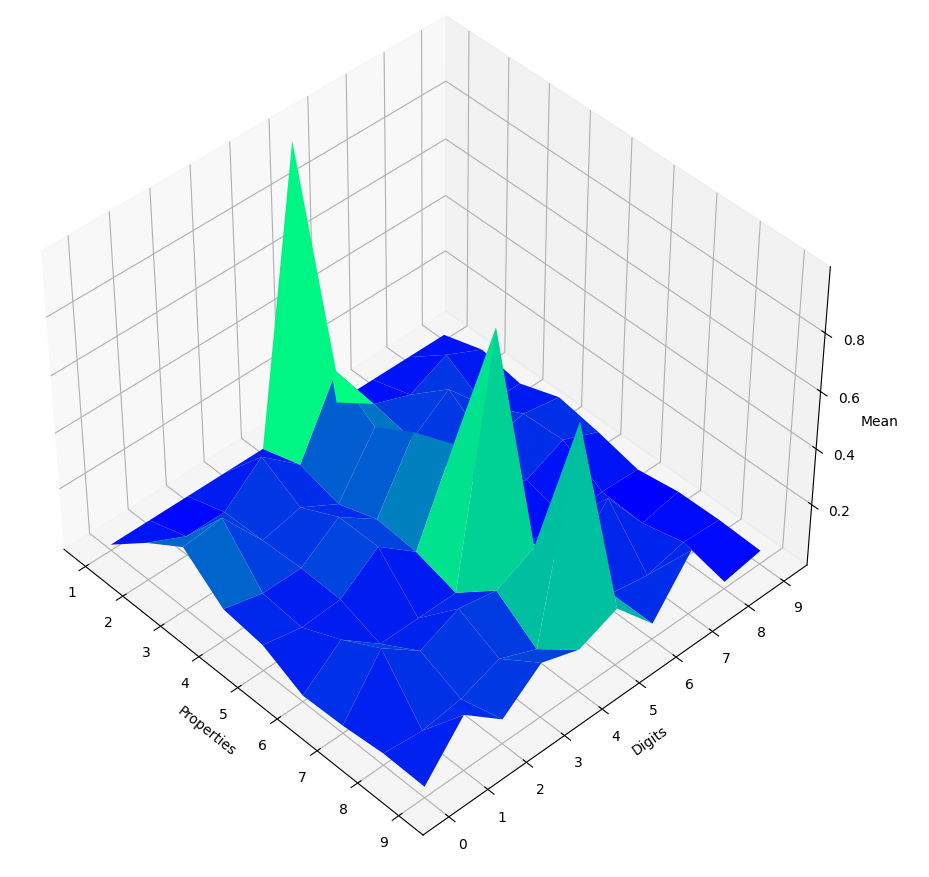
\includegraphics[width=70mm]{./images/digit-5.png}}
\caption{Mean property NNA output for the digit 5}
\label{digit5votes}
\end{figure}

\begin{figure}[htbp]
\centerline{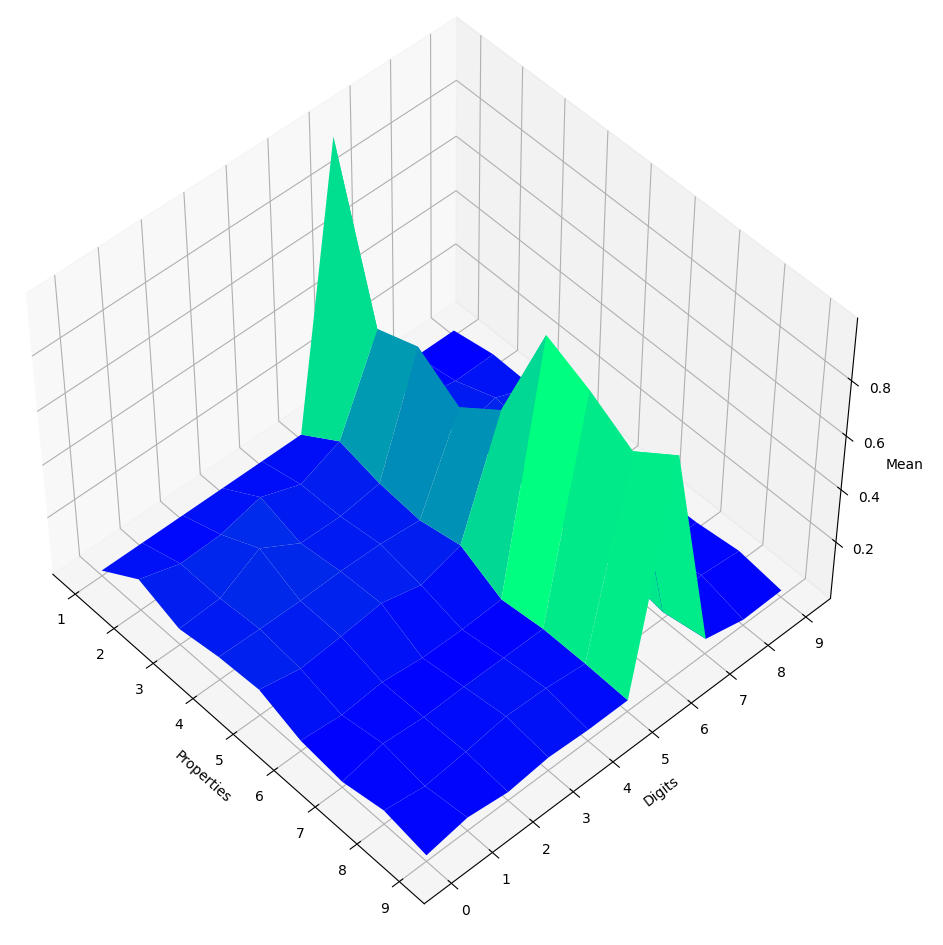
\includegraphics[width=70mm]{./images/digit-6.png}}
\caption{Mean property NNA output for the digit 6}
\label{digit6votes}
\end{figure}

%\begin{table}[htbp]
%\caption{Properties, Transforms and Property Identifiers}
%\centering
%\begin{tabular}{| c | c | c |}
%\hline
% Identifier & Explainable Property & Transform \\
%\hline\hline
%$P_1$ & Stroke & Skeleton \\
%\hline
%$P_x$ & Circle & Hough Circle \\
%\hline
%$P_x$ & Crossings & Crossing Point \\
%\hline
%$P_x$ & Ellipse & Hough Ellipse \\
%\hline
%$P_x$ & Ellipse + Circle & Hough Ellipse and Circle \\
%\hline
%$P_x$ & Endpoints & Endpoints \\
%\hline
%$P_x$ & Enclosed Region & Flood Fill \\
%\hline
%$P_x$ & Line & Hough Line \\
%\hline
%$P_x$ & Enclosed Region of Skeleton & Skeleton Flood Fill \\
%\hline
%\end{tabular}
%\label{table:tblproptrans}
%\end{table}

 \begin{figure}[htbp]
\centerline{
\includegraphics[width=15mm]{./digit-images/5-0.png}}
\caption{Example 1 of a handwritten digit five}
\label{example1}
\end{figure}

We next present three interesting MNIST digits and review the property classifications, property effectiveness, and explainability.  Stepping through the procedures of the probabilistic voting scheme, we show the classification results for the digits as well as the explainability rationale from XAI as well as the confidence.

\begin{table}[htbp]
\caption{Probabilistic voting and explainability for Example 1}
\centering
\begin{tabular}{| c | c | c | c | p{0.08\linewidth} | p{0.08\linewidth} |}
\cline{3-6}
\multicolumn{2}{c}{} & \multicolumn{2}{|c|}{Effectiveness} & \multicolumn{2}{c|}{Explainability} \\
\hline
 Prop. & Vote & $E_{i,5}$ & $E_{i,6}$ & $X_5$ & $X_6$ \\
\hline \cline{0-5}
$P_1$ & 5 & 1.000 & - & \checkmark & - \\ 
\hline
$P_2$ & 6 & - & 0.465 & - & \checkmark \\
\hline
$P_3$ & - & - &  - & - & - \\
\hline
$P_4$ & - & - & - & - & - \\
\hline
$P_5$ & 6 & - & 0.490 & - & \checkmark \\
\hline
$P_6$ & 5 & 0.854 & - & \checkmark & - \\
\hline
$P_7$ & - & - & - & - & - \\
\hline
$P_8$ & 5 & 0.700 & - & \checkmark & - \\
\hline
$P_9$ & - & - & - & - & - \\
\hline \cline{0-5}
\multicolumn{2}{|c|}{Weight Totals} & $2.554$ & $0.955$ & \multicolumn{2}{c|}{$\sum W_\gamma=3.509$} \\
\cline{0-5}
\multicolumn{2}{|c|}{Confidence} & $73\%$ & $24\%$ & \multicolumn{2}{c}{} \\
\cline{0-3}
\end{tabular}
\label{table:example1}
\end{table}

The first example  digit, labeled a five, is shown in Fig.~\ref{example1}.  Voting and explainability is detailed in Table ~\ref{table:example1}.  The property votes for this example are shown in the Vote column.  Cells with dashes are properties that did not have a sufficiently strong opinion on a particular digit, i.e., no class was above a threshold.   The $E_{i,x}$ columns give the effectiveness of a property $i$ to correctly select class $x$.  The effectiveness values are from the knowledgebase using eq. (\ref{effectiveness}).   The stroke $(P_1)$, endpoint $(P_6)$ and line $(P_8)$ properties suggest the digit is a five with effectiveness $E_{1,5}= 1.000$, $E_{6,5}=0.854$, and $E_{8,5}=0.700$.  Weight of effectiveness for the digit five is $W_5=2.554$, given by eq. (\ref{weight}).  The circle $(P_2)$ and $(P_5)$ properties suggest that the digit is a six with effectiveness $E_{2,6}=0.465$ and $E_{5,6}=0.490$  and a weight of $W_6=0.955$.  Taking the sum of the total weights, $\sum\limits_\gamma W_\gamma=3.509$.  Confidence, as given by eq. (\ref{conf}), for the five, is given as $C_5=\frac{2.554}{3.509} = 73\%$.  Alternatively, six was suggested by properties where confidence is $C_6=\frac{0.955}{3.509}=27\%$.  Five wins because $C_6=27\% < 73\%=C_5$.  We also observe that the explainability, $X_x$, columns provide rationale for each of the classes that were selected based on the selecting properties.   E.g.,  the logic in the XAI block references property information from explainability column $X_5$ and assembles rationale indicating that the five was selected because the stroke, endpoint, and line properties are consistent with a five. 

 \begin{figure}[htbp]
\centerline{
\includegraphics[width=15mm]{./digit-images/9-9.png}}
\caption{Example 2 of a handwritten digit nine}
\label{example2}
\end{figure}

%\begin{table}[htbp]
%\caption{Property Votes for Example 2}
%\centering
%\begin{tabular}{| c | c | c |}
%\hline
% Property Id & Vote & Weight \\
%\hline\hline
%$P_0$ & 9 & 1.000 \\ 
%\hline
%$P_1$ & 3 & 0.327 \\
%\hline
%$P_2$ & 5 & 0.057 \\
%\hline
%$P_3$ & - & - \\
%\hline
%$P_4$ & - & - \\
%\hline
%$P_5$ & 6 & 0.932 \\
%\hline
%$P_6$ & 9 & 0.809 \\
%\hline
%$P_7$ & - & - \\
%\hline
%$P_8$ & 9 & 0.821 \\
%\hline
%\end{tabular}
%\label{table:example2}
%\end{table}

The second example,  labeled a nine, is shown in Fig.~\ref{example2}.  Table ~\ref{table:example2} shows the property predictions, voting results, and rationale for example 3.  In this example three properties selected the digit nine and three other properties selected the digits three, five, and six.  The results from the voter for this example were that nine was selected by the voter with a $67\%$ confidence and an explanation that the stroke and enclosed region properties were consistent with those of a nine.  We noted on this example that it is surprising that none of the properties indicated an eight because of the example's similarity to a digit eight.  

 \begin{figure}[htbp]
\centerline{
\includegraphics[width=15mm]{./digit-images/2-4.png}}
\caption{Example 3 of a handwritten digit two}
\label{example3}
\end{figure}

%\begin{table}[htbp]
%\caption{Property Votes for Example 3}
%\centering
%\begin{tabular}{| c | c | c |}
%\hline
% Property Id & Vote & Weight \\
%\hline\hline
%$P_0$ & 2 & 1.000 \\ 
%\hline
%$P_1$ & 3 & 0.327 \\
%\hline
%$P_2$ & - & - \\
%\hline
%$P_3$ & 2 & 0.161 \\
%\hline
%$P_4$ & 3 & 0.387 \\
%\hline
%$P_5$ & 2 & 0.938 \\
%\hline
%$P_6$ & - & - \\
%\hline
%$P_7$ & 2 & 0.639 \\
%\hline
%$P_8$ & - & - \\
%\hline
%\end{tabular}
%\label{table:example3}
%\end{table}

\begin{table}[htbp]
\caption{Probabilistic voting and explainability for Example 3}
\centering
\begin{tabular}{| c | c | c | c | p{0.08\linewidth} | p{0.08\linewidth} |}
\cline{3-6}
\multicolumn{2}{c}{} & \multicolumn{2}{|c|}{Effectiveness} & \multicolumn{2}{c|}{Explainability} \\
\hline
 Prop. & Vote & $E_{i,2}$ & $E_{i,3}$ & $X_2$ & $X_3$ \\
\hline \cline{0-5}
$P_1$ & 2 & 1.000 & - & \checkmark & - \\ 
\hline
$P_2$ & 3 & - & 0.327 & - & \checkmark \\
\hline
$P_3$ & - & - &  - & - & - \\
\hline
$P_4$ & 2 & 0.161 & - & \checkmark & - \\
\hline
$P_5$ & 3 & - & 0.387 & - & \checkmark \\
\hline
$P_6$ & 2 & 0.938 & - & \checkmark & - \\
\hline
$P_7$ & - & - & - & - & - \\
\hline
$P_8$ & 2 & 0.639 & - & \checkmark & - \\
\hline
$P_9$ & - & - & - & - & - \\
\hline \cline{0-5}
\multicolumn{2}{|c|}{Weight Totals} & $2.738$ & $0.714$ & \multicolumn{2}{c|}{$\sum W_\gamma=3.452$} \\
\cline{0-5}
\multicolumn{2}{|c|}{Confidence} & $79\%$ & $21\%$ & \multicolumn{2}{c}{} \\
\cline{0-3}
\end{tabular}
\label{table:example3}
\end{table}

The third example handwritten digit, labeled a two, is shown in Fig. ~\ref{example3} and Table ~\ref{table:example3}.  In this case,  the voter selects the digit two with a $79\%$ confidence due to stroke, circle, endpoint, and line properties consistent with the digit two.  A three was suggested with $21\%$ confidence due to circle properties.  We noted in this example that classification results from circle properties had conflicting votes.  $P_2$ and $P5$ voted for three while $P_4$ voted for two.

\begin{table}[htbp]
\caption{NNA Voter results for examples}
\centering
\begin{tabular}{| c | c | c | c |}
\hline
 Digit & Ex. 1 & Ex. 2 & Ex. 3 \\
\hline\hline
0 & 1.92e-06 & 1.11e-08 & 2.98e-07\\ 
\hline
1 & 1.44e-06 & 1.52e-07 & 1.93e-08 \\
\hline
2 & 1.40e-06 & 4.54e-09 & \textbf{9.99e-01} \\
\hline
3 & 5.12e-08 & 2.48e-04 & 5.26e-06 \\
\hline
4 & 1.79e-08 & 1.33e-06 & 5.91e-06 \\
\hline
5 & \textbf{9.99e-01} & 2.31e-07 & 1.41e-06 \\
\hline
6 & 7.69e-07 & 2.23e-04 & 5.83e-07 \\
\hline
7 & 4.88e-07 & 4.93e-08 & 1.89e-09 \\
\hline
8 & 2.47e-07 & 5.71e-06 & 5.51e-07 \\
\hline
9 & 5.21e-07 & \textbf{9.99e-01} & 1.71e-08 \\
\hline
\end{tabular}
\label{table:nnavoter}
\end{table}

Table~\ref{table:nnavoter} shows the output of the ML voting scheme on the three examples.  The ten rows in the table represent the corresponding digits.  The columns for examples 1 through 3 contain the values output by the voter NNA when presented with the property votes from the examples.  We observe that in each example the ML Voter overwhelmingly selects the appropriate digit shown in bold.

\section{Results}

We introduce two metrics to compare aggregate results from the two voting schemes.  The first metric is Identification Accuracy which gauges the correctness of the system in performing classification.  Identification Accuracy is the ratio of the number of correct classifications to the total number of classifications of the voter model engine.  The second metric, Explainability Quality, is used to estimate the correspondence or connection of explanations with classification decisions.  Explainability Quality is the ratio of classifications decisions with at least one property justifying the classification by the voter scheme to the total number of classifications.   In both metrics, values close to one are desired.

Results for Identification Accuracy obtained using the probabilistic voting scheme on the MNIST dataset were $0.919$ while results obtained from the NNA voting scheme were $0.959$.  Results for Explainability Quality using the probabilistic voter scheme were $1.00$ while results for the NNA voting scheme were $0.982$.

The ML voter scheme was more accurate in classifying input than the probabilistic scheme by about 4\%.   However, the probabilistic voter scheme was nearly 2\% better in terms of Explainability Quality over the ML voting scheme.  Note that in the probabilistic scheme, the voter model engine selects a class from among the property votes, so there is always a property that corresponds to the voter output.  The NNA in the ML voting scheme is trained based on labels on the training set which may not correspond to a vote from a property in a small percentage of inputs.

It appears there can be cases where identification accuracy and explanation quality may not be well balanced.  The particulars of the application will need to be considered.  It is our view that, in some applications, the quality of explainability may have greater importance than identification accuracy.

\begin{table*}[htbp]
\caption{Probabilistic voting and explainability for Example 2}
\centering
\begin{tabular}{| c | c | c | c | c | c | c | c | c | c |}
\cline{3-10}
\multicolumn{2}{c}{} & \multicolumn{4}{|c|}{Effectiveness} & \multicolumn{4}{c|}{Explainability} \\
\hline
 Prop. & Vote & $E_{i,3}$ & $E_{i,5}$ & $E_{i,6}$ & $E_{i,9}$ & $X_3$ & $X_5$ & $X_6$ & $X_9$ \\
\hline \cline{0-9}
$P_1$ & 9 & - & - & - & 1.00 & - & - & - & \checkmark \\ 
\hline
$P_2$ & 3 & 0.327 & - & - & - & \checkmark & - & - & - \\
\hline
$P_3$ & 5 & - &  0.057 & - & - & - & \checkmark & - & - \\
\hline
$P_4$ & - & - & - & - & - & - & - & - & - \\
\hline
$P_5$ & - & - & - & - & - & - & - & - & - \\
\hline
$P_6$ & 6 & - & - & 0.933 & - & - & - & \checkmark & - \\
\hline
$P_7$ & 9 & - & - & - & 0.809 & - & - & - & \checkmark \\
\hline
$P_8$ & - & - & - & - & - & - & - & - & - \\
\hline
$P_9$ & 9 & - & - & - & 0.821 & - & - & - & \checkmark \\
\hline \cline{0-9}
\multicolumn{2}{|c|}{Weight} & 0.327 & 0.057 & 0.933 & 2.630 & \multicolumn{4}{c|}{$\sum W_\gamma=3.946$} \\
\cline{0-9}
\multicolumn{2}{|c|}{Confidence} & $8\%$ & $1\%$ & $24\%$ & $67\%$ & \multicolumn{4}{c}{} \\
\cline{0-5}
\end{tabular}
\label{table:example2}
\end{table*}

\begin{table*}
\caption{Digit 5 Outputs}
\centering\begin{tabular}{ | c ||  c | c | c | c | c | c | c | c | c |}
 digit 5 & $P_1$ & $P_2$ & $P_3$ & $P_4$ & $P_5$ & $P_6$ & $P_7$ & $P_8$ & $P_9$ \\
\hline \hline
effectiveness $E_{i,5}$  & 100.0 & 14.2 & 5.7 & 20.8 & 21.5 & 85.4 & 3.8 & 70.0 & 5.5 \\
\hline
$\sigma$ & 0.300& 0.076& 0.082& 0.068& 0.089& 0.252& 0.074& 0.211& 0.077 \\
\hline
k & 10.000& 3.995& -1.864& 5.555& 6.229& 9.550& -1.941& 9.779& -2.063 \\
\hline
skew & 3.162& 1.913& 0.330& 2.324& 2.413& 3.073& -0.025& 3.116& 0.061 \\
\hline
0 & 0.000 & 0.115 & 0.208 & 0.093 & 0.073 & 0.002 & 0.007 & 0.023 & 0.020 \\
\hline
1 & 0.000 & 0.048 & 0.223 & 0.057 & 0.044 & 0.111 & 0.193 & 0.008 & 0.183 \\
\hline
2 & 0.000 & 0.048 & 0.051 & 0.058 & 0.053 & 0.001 & 0.089 & 0.027 & 0.069 \\
\hline
3 & 0.000 & 0.162 & 0.082 & 0.154 & 0.154 & 0.002 & 0.149 & 0.079 & 0.178 \\
\hline
4 & 0.000 & 0.046 & 0.006 & 0.056 & 0.045 & 0.003 & 0.122 & 0.019 & 0.130 \\
\hline
5 & 1.000 & 0.300 & 0.200 & 0.284 & 0.345 & 0.849 & 0.186 & 0.732 & 0.185 \\
\hline
6 & 0.000 & 0.097 & 0.069 & 0.059 & 0.090 & 0.009 & 0.027 & 0.036 & 0.037 \\
\hline
7 & 0.000 & 0.045 & 0.167 & 0.067 & 0.041 & 0.001 & 0.185 & 0.011 & 0.212 \\
\hline
8 & 0.000 & 0.109 & 0.022 & 0.094 & 0.101 & 0.014 & 0.005 & 0.042 & 0.005 \\
\hline
9 & 0.000 & 0.044 & 0.019 & 0.069 & 0.043 & 0.009 & 0.032 & 0.034 & 0.028 \\
\hline
false positive \%  & 0.0 & 0.5 & 0.2 & 0.4 & 0.7 & 0.4 & 0.0 & 0.3 & 0.0 \\
\hline
false negative \%  & 0.0 & 84.8 & 94.1 & 78.8 & 78.3 & 13.4 & 96.2 & 29.2 & 94.5 \\
\hline
\end{tabular}
\label{table:digit5out}
\end{table*}

\begin{table*}
\caption{Digit 6 Outputs}
\centering\begin{tabular}{ | c ||  c | c | c | c | c | c | c | c | c |}
 digit 6 & $P_1$ & $P_2$ & $P_3$ & $P_4$ & $P_5$ & $P_6$ & $P_7$ & $P_8$ & $P_9$ \\
\hline \hline
effectiveness $E_{i,6}$  & 100.0 & 46.5 & 49.5 & 32.0 & 49.0 & 93.3 & 81.8 & 70.7 & 83.2 \\
\hline
$\sigma$ & 0.300& 0.112& 0.130& 0.094& 0.133& 0.264& 0.240& 0.209& 0.246 \\
\hline
k & 10.000& 8.507& 8.617& 9.864& 9.469& 9.955& 9.935& 9.889& 9.930 \\
\hline
skew & 3.162& 2.842& 2.886& 3.132& 3.048& 3.153& 3.148& 3.138& 3.147 \\
\hline
0 & 0.000 & 0.100 & 0.042 & 0.069 & 0.080 & 0.020 & 0.001 & 0.034 & 0.004 \\
\hline
1 & 0.000 & 0.052 & 0.050 & 0.066 & 0.048 & 0.005 & 0.035 & 0.011 & 0.033 \\
\hline
2 & 0.000 & 0.057 & 0.135 & 0.064 & 0.061 & 0.020 & 0.022 & 0.028 & 0.013 \\
\hline
3 & 0.000 & 0.095 & 0.046 & 0.070 & 0.079 & 0.002 & 0.027 & 0.051 & 0.032 \\
\hline
4 & 0.000 & 0.039 & 0.044 & 0.067 & 0.040 & 0.000 & 0.027 & 0.046 & 0.023 \\
\hline
5 & 0.000 & 0.101 & 0.065 & 0.052 & 0.086 & 0.008 & 0.028 & 0.029 & 0.024 \\
\hline
6 & 1.000 & 0.426 & 0.482 & 0.380 & 0.495 & 0.890 & 0.818 & 0.725 & 0.837 \\
\hline
7 & 0.000 & 0.057 & 0.049 & 0.077 & 0.047 & 0.000 & 0.033 & 0.007 & 0.038 \\
\hline
8 & 0.000 & 0.027 & 0.086 & 0.068 & 0.030 & 0.034 & 0.004 & 0.041 & 0.001 \\
\hline
9 & 0.000 & 0.029 & 0.026 & 0.077 & 0.038 & 0.000 & 0.007 & 0.027 & 0.005 \\
\hline
false positive \%  & 0.0 & 2.6 & 2.5 & 0.5 & 2.2 & 0.7 & 0.2 & 0.6 & 0.0 \\
\hline
false negative \%  & 0.0 & 53.3 & 50.1 & 67.5 & 50.7 & 6.6 & 18.1 & 28.1 & 16.8 \\
\hline
\end{tabular}
\label{table:digit6out}
\end{table*}

%\section{References}
\bibliographystyle{plain}
\bibliography{references}{}


\end{document}
